\section{EXPERIMENTS} \label{sec:experiments}

In this section a numerical results of the validation benchmark and
  optimization of a photoinjector operated in the space charge dominated regime is presented.

\subsection{Optimizer Validation}

\begin{figure}
    \centering
    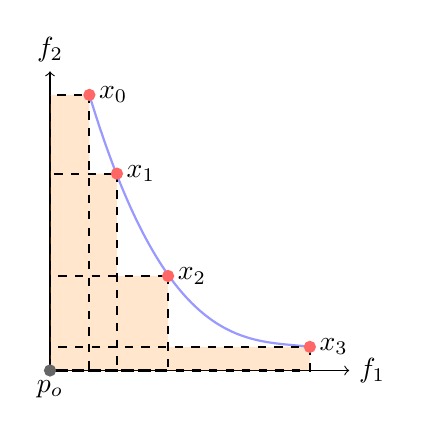
\begin{tikzpicture}[text=black]
      \coordinate (y) at (0,3.8);
\coordinate (x) at (3.8,0);
\draw[<->] (y) node[above] {$f_2$} -- (0,0) --  (x) node[right]
{$f_1$};

\path
  coordinate (start) at (0.5,3.5)
  coordinate (c1) at +(1.5,0.2)
  coordinate (c2) at +(2.5,0.4)
  coordinate (top) at (3.3,0.3);

\draw [thick, blue!40!white] (start) .. controls (c1) and (c2) .. (top);
(start) .. controls (c1) and (c2) .. (top) -- (3.3,0.0);
%\draw [fill, color=blue, draw opacity=0, fill opacity=0.2] (0,0) -- (0.0, 3.5) --
%(start) .. controls (c1) and (c2) .. (top) -- (3.3,0.0);


\draw[fill, color=orange, draw opacity=0, fill opacity=0.2] (0,0) -- (0, 3.5) --
(start) -- (0.5,2.5) -- (0.85, 2.5) -- (0.85, 1.2) -- (1.5, 1.2) -- (1.5, 0.3) -- (top) -- (3.3, 0.0);
\draw[dashed, thick] (start) rectangle (0,0);
\draw[dashed, thick] (top) rectangle (0,0);
\draw[dashed, thick] (0.85,2.5) rectangle (0,0);
\draw[dashed, thick] (1.5,1.2) rectangle (0,0);

\filldraw [red!60!white]
(start) circle (2pt) node[right, black] {$x_0$}
(0.85,2.5) circle (2pt) node[right, black] {$x_1$}
(1.5,1.2) circle (2pt) node[right, black] {$x_2$}
(top) circle (2pt) node[right, black] {$x_3$};

\filldraw [black!60!white]
(0,0) circle (2pt) node[below, black] {$p_o$};


    \end{tikzpicture}
  \caption{The hypervolume for a two-objective optimization problem
  corresponds to the shaded area formed by the dashed rectangles spanned by
  all points on the Pareto front and an arbitrary selected origin $p_o$.}
  \label{fig:hypervolume}
\end{figure}

To ensure that the optimizer works correctly the benchmark
  problem (\ref{eqn:bench}) was solved.
To that end, we use a metric for comparing the quality of a Pareto
  front.
Given a point in the Pareto set, we compute the $m$ dimensional volume (for
  $m$ objectives) of the dominated space, relative to a chosen origin.
This is visualized for $2$ objectives in Fig.~\ref{fig:hypervolume}.
For further information and details of the implementation see~\cite{whbb:12}.
Figure~\ref{fig:pisa_bench} and the corresponding hypervolume values in
  Table~\ref{tbl:bench_rms_error}, show expected convergence.
The reference Pareto front is clearly very well approximated.
It took a total of 1100 function evaluations to perform this computation.
The hypervolume of the reference solution ($0.6575$) for our benchmark was
  computed by sampling the solution provided in~\cite{hbwh:05}.

\begin{figure}
  \centering
    \includegraphics[width=0.7\linewidth]{figures/valid_front}
  \caption{Variator benchmark after $1100$ function evaluations using binary
           crossover and independent gene mutations (each gene mutates with
           probability $p=\frac{1}{2}$) on a population of $100$
           individuals.}
  \label{fig:pisa_bench}
\end{figure}

\begin{table}%[h!]
\begin{center}
  \caption{Convergence of benchmark problem with errors relative to
    hypervolume of sampled reference solution.}
  \label{tbl:bench_rms_error}
  \begin{tabular}{c|c|c}
    \hline\noalign{\smallskip}
    tot.\ function  & hyper volume & relative error\\
    evaluations    & & \\
    \noalign{\smallskip}\hline\noalign{\smallskip}
    100  &  0.859753 & $3.076 \times 10^{-1}$ \\
   % \noalign{\smallskip}\hline\noalign{\smallskip}
    200  &  0.784943 & $1.938 \times 10^{-1}$ \\
    500  &  0.685183 & $4.210 \times 10^{-2}$ \\
    900  &  0.661898 & $6.689 \times 10^{-3}$ \\
    1100 &  0.657615 & $1.749 \times 10^{-4}$ \\
    \noalign{\smallskip}\hline
  \end{tabular}
\end{center}
\end{table}

Table~\ref{tbl:bench_rms_error} shows satisfactory
  convergence to the sampled reference Pareto front after 1000 (plus the
  additional 100 evaluations for the initial population) function evaluations.



\subsection{AWA Photoinjector Optimization} \label{awaproblem}
Next the optimization framework is applied to a high charge beam line
 at the Argonne Wakefield Accelerator (AWA) facility. 
The goal of this optimization is to produce beams of electrons that meet 
design specifications; this includes number of particles (charge), energy, and particle distribution (characterized by beam sizes and energy spread).
As shown in Fig.~\ref{awa-linac}, the installed portion of the the 
beam line consists of an rf photocathode gun, 
two solenoids, and six linear accelerating cavities
followed by four quadrupoles and a stripline kicker. 
The charge of interest, 40 nC, is needed for Two Beam 
Acceleration (TBA) 
experiments performed at AWA \cite{gai_power_jing_2012,JING201872}, 
which motivates this work. 
Prior experimental results were limited by beam size when the beam passed through small aperture 
wakefield structures located downstream. 
In an attempt to maximize charge transmission in upcoming experiments,
magnet strengths of the solenoids and quadrupoles leading into the 
TBA section of the beam line were optimized, shown in Fig.~\ref{awa-tba}.
The simulation model includes from the gun to the septum.
The optimization location is chosen as the  
entrance to the first quadrupole on the dog leg ($s_3$), see Fig.~\ref{awa-tba}.
Minimizing beam sizes here will enable capture and further focusing before space charge effects dominate the beam. 
This will also enable cleaner transport through downstream elements.
%\vspace{-1em}

\def \gunheight {25}  %25} %double sided number
\def \quadheight {35}
\def \quadleft {115}  %127} %double sided number
\def \kickerleft {145}  %160} % two sided number
\def \leftarrow{10}
\def \bottomofarrows {29}
\def \topofarrows {34}
\begin{figure*}
	\begin{tikzpicture}[every node/.style={anchor=south west,inner sep=0pt},x=1mm, y=1mm,]   
	\node (fig1) at (0,0)
	{\includegraphics[width=\textwidth]{figures/awa-drawing}};
	\node[fill=white, inner sep=2pt] (txt2) at (0,\gunheight) {\large Gun};
	\node[fill=white, inner sep=2pt] (txt2) at (20,\gunheight) {\large Accelerating Cavities};
	\node[fill=white, inner sep=2pt] (txt2) at (\quadleft-5,\quadheight) {\large Quadrupoles};
	\draw [blue, ->, line width=1] (\quadleft+\leftarrow,\topofarrows) -- (\quadleft+\leftarrow, \bottomofarrows);
	\node[fill=white, inner sep=2pt] (txt2) at (\kickerleft,20) {\large $s_1$};
	\node[fill=white, inner sep=2pt] (txt2) at (\kickerleft+8,20) {\large $s_2$};
	\node[fill=white, inner sep=2pt] (txt2) at (\kickerleft,\quadheight) {\large Kicker};
	\draw [blue, ->, line width=1] (\kickerleft+\leftarrow-3,\topofarrows) -- (\kickerleft+\leftarrow-3, \bottomofarrows);	
	\draw [black, ->, line width=1] (0,-2) -- (100, -2);
	\node[fill=white, inner sep=2pt] (txt2) at (50,0) {\large Beam Direction};
	\end{tikzpicture}
	\caption{Side view of the high charge linac at the AWA. 
		All hardware in this drawing is currently installed. 
	Note locations $s_1$ and $s_2$, before and after the kicker.}
	\label{awa-linac}
	%\vspace{-7em}
\end{figure*}

\def \septheight {65}
\def \bottomarrow {55} %57}
\def \kleft {13}
\def \sleft {38}%41.5}
\def \sheight {45}%47}
\def \beam {35}
\begin{figure*}
	\begin{tikzpicture}[every node/.style={anchor=south west,inner sep=0pt},x=1mm, y=1mm,]   
	\node (fig2) at (0,0)
	{\includegraphics[width=\textwidth]{figures/tba_dogleg}};
	\node[fill=white, inner sep=2pt] (txt2) at (3,\sheight) {\large $s_1$};
	\node[fill=white, inner sep=2pt] (txt2) at (20,\sheight) {\large $s_2$};
	\node[fill=white, inner sep=2pt] (txt2) at (41,40) {\large $s_3$}; %(46,45)
	\node[fill=white, inner sep=2pt] (txt2) at (33,\septheight) {\large Septum};
	\draw [blue, ->, line width=1] (\sleft,\septheight) -- (\sleft, \bottomarrow);	
	\node[fill=white, inner sep=2pt] (txt2) at (7,\septheight) {\large Kicker};
	\draw [blue, ->, line width=1] (\kleft,\septheight) -- (\kleft, \bottomarrow);
	\draw [black, ->, line width=1] (0,\beam) -- (100,\beam);
	\node[fill=white, inner sep=2pt] (txt2) at (50,\beam+2) {\large Beam Direction};
	\end{tikzpicture}
	\vspace{-12em}
	\caption{Continuation of the high charge beam line layout at the AWA, top view. 
		This is the proposed two beam acceleration section. 
		Only the kicker in this drawing is installed. 
	Note $s_3$, the entrance to the fifth quadrupole on the beam line.
	This is the optimization location.}
	\label{awa-tba}
\end{figure*}
%
%\vspace{-1em}

In addition to addressing the challenge of producing an optimized beam, 
this model was chosen to demonstrate the ability of the framework to tackle large problems.
Six design variables and objectives were used, along with three constraints.
The objectives include transverse and longitudinal beam sizes, 
transverse momentum, and longitudinal energy spread. 
The design variables include the two gun solenoids and 
the first four quadrupoles strengths. 
This problem encompasses high dimensionality 
and nonlinear effects such as space charge. There is no existing information
that accurately predicts optimized parameters for this beam line. 
This work is meaningful in that it will guide future operations at the AWA.


\subsubsection{Time Step Scan} \label{awa:subsection:test}
Before running a full scale optimization of the problem described in Subsection \ref{awaproblem}, 
a study on time step and number of particles in the simulation model 
was done to reduce the time of the simulation while 
maintaining the physics of interest. 
The grid size $16 \times 16 \times 32$ was chosen, 
and parallelized in the x and y directions.
After comparing several options (1,000, 10,000, 20,000, 50,000, 100,000) 
with a small time step, the number of particles was fixed at 10,000.
Next several time steps were explored, see Table~\ref{timestep}.
The largest steps were too big to resolve the beam parameters accurately.
See low fidelity plot in Fig.~\ref{tstep} for $dT=$\num{5E-11} results.  

\begin{table}%[h!]
	\begin{center}
		\caption{Checkmarks (\cmark) indicate desired beam parameters are resolved at that time step. 
			An (\xmark) indicates the time step is too large, and results are nonphysical.}
		\label{timestep}
		\begin{tabular*}{0.48\textwidth}{c @{\extracolsep{\fill}} C c D }
			\hline\noalign{\smallskip}
			Time Step (dT) & Linac & Drift & Quadrupoles \\
			\noalign{\smallskip}\hline\noalign{\smallskip}
			$5 \times10^{-10}$  & \xmark & \xmark & \xmark \\
			$1 \times10^{-10}$  & \xmark & \xmark & \xmark \\
			$5 \times10^{-11}$  & \xmark & \xmark & \xmark \\
			$1 \times10^{-11}$  & \cmark & \cmark & \xmark \\
			$5 \times10^{-12}$  & \cmark & \cmark & \xmark \\
			$1 \times10^{-12}$  & \cmark & \cmark & \cmark \\
			\noalign{\smallskip}\hline
		\end{tabular*}
	\end{center}
\end{table}

In the drifts and linac tanks, $dT=\num{1E-11}$ was sufficient. 
However, it was not acceptable near the quadrupoles. 
For all models, the longitudinal parameters (rms$_s$ and energy) 
are calculated correctly, but discrepancies are seen in the transverse 
(rms$_x$ and $\epsilon_x$) for low fidelity results. This discrepancy is 
what led to the decision to adjust the time steps w.r.t. beam line elements. 
In the linac and drift sections $dT=\num{1E-11}$ was used. 
Near sensitive elements such as the quadrupoles, kicker, and septum, 
a time step of $dT=\num{1E-12}$ was used.
The resulting simulations are low fidelity in most places, but closely approximate 
the mid fidelity simulations for metrics of interest, as shown in 
Fig.~\ref{tstep}.  Mid fidelity simulations used steps of  $dT=\num{1E-12}$ everywhere.
The average run time of each simulation with the adjusted time steps was 1.6~minutes.
In comparison, the mid fidelity simulation ran for 18~minutes.
Note, a smaller time step, \num{1E-13}, is always used in the gun where the 
beam has low energy and changing rapidly.
%A summary of the parameters used is listed in Table \ref{fidelity}. 

\begin{figure}%[h]
	\centering
	\includegraphics[width=\linewidth]{figures/timestep_comparison_paper}
	\caption{Comparison of different fidelity models (dT stands for time step).}
	\label{tstep}
\end{figure}

\subsubsection{Hyper parameter Scan}
While the optimization problem and goals were well defined (Subsection \ref{awaproblem}), 
it was not clear what the best hyper parameters for the genetic algorithm would be.
These parameters include gene mutation probability, mutation probability, 
recombination probability, number of individuals, 
and number of generations to complete. 
Given the beam line in Fig.~\ref{awa-linac},
four small optimization experiments were done with various hyper parameters. 
Similar to the time step scan, 
the goal of this exercise was to determine which set of optimization
parameters strongly influence the results, 
and whether there was a time to solution difference.
From here on, we will reference each experiment as ex-1, ex-2, ex-3, and ex-4
as shown in Table \ref{extable}. 
\begin{table}%[h!]
	\begin{center}
		\caption{Input Parameters for initial twenty four hour AWA optimization experiments. 
			The gene mutation probability was equal to the mutation probability (not shown) in all four experiments. 
			The max number of individuals per generation was~80.}
		\label{extable}
		\begin{tabular*}{0.48\textwidth}{l @{\extracolsep{\fill}} C C D }
			\hline\noalign{\smallskip}
			& Gene Mutation Probability & Recombination Probability & Number of completed generations \\
			\noalign{\smallskip}\hline\noalign{\smallskip}
			ex-1 &  0.1  & 0.9  &  96 \\
			ex-2 &  0.3  & 0.7  &  81 \\
			ex-3 &  0.8  & 0.2  &  53 \\
			ex-4 &  0.01 & 0.09 &  95 \\
			\noalign{\smallskip}\hline
		\end{tabular*}
	\end{center}
\end{table}


The maximum number of individuals per generation was fixed at 80. 
This number was chosen based on the node architecture, and the 
to prevent a prohibitive computational cost.  
Each experiment was allowed to run for twenty four hours, with 
a maximum generation limit of 100. 
We reduced the six objectives to four, 
and shortened the simulation time by moving the objectives further 
upstream to $s_1$ and $s_2$, the locations before and after the kicker, 
see Fig.~\ref{awa-tba}.  


The objectives include: $\varepsilon_{x}\left(s = s_1\right)\text{, } \varepsilon_{x}\left(s = s_2\right)$, $\text{rms}_{s}\left(s = s_1\right)\text{, and }  \text{rms}_{s}\left(s = s_2\right)$. 
The OPAL input file for ex-3 is given as an example to show how optimization and design variables are defined:

\iffalse
%\vspace{0.2cm}
\begin{samepage}
	\begin{Verbatim}[fontsize=\scriptsize]
	OPTION, ECHO=FALSE;
	OPTION, INFO=TRUE;
	
	TITLE, STRING="ANL Optimization";
	
	dv0: DVAR, VARIABLE="IBF",    LOWERBOUND=200.0, UPPERBOUND=500.0;
	dv1: DVAR, VARIABLE="IM",     LOWERBOUND=170.0, UPPERBOUND=260.0;
	dv2: DVAR, VARIABLE="GPHASE", LOWERBOUND=-30.0, UPPERBOUND=0.0;
	dv3: DVAR, VARIABLE="FWHM",   LOWERBOUND=1.5,   UPPERBOUND=10.0;
	
	// Quad values
	dv4: DVAR, VARIABLE="KQ1", LOWERBOUND=-8.0, UPPERBOUND=8.0;
	dv5: DVAR, VARIABLE="KQ2", LOWERBOUND=-8.0, UPPERBOUND=8.0;
	dv6: DVAR, VARIABLE="KQ3", LOWERBOUND=-8.0, UPPERBOUND=8.0;
	dv7: DVAR, VARIABLE="KQ4", LOWERBOUND=-8.0, UPPERBOUND=8.0;
	
	rmss1:  OBJECTIVE,EXPR="fabs(statVariableAt('rms_s',16.5))";
	emitx1: OBJECTIVE,EXPR="fabs(statVariableAt('emit_x',16.5))";
	
	rmss2:  OBJECTIVE,EXPR="fabs(statVariableAt('rms_s',18.5))";
	emitx2: OBJECTIVE,EXPR="fabs(statVariableAt('emit_x',18.5))";
	
	c1: CONSTRAINT, EXPR="fabs(statVariableAt('rms_x',16.5))<1.0e-1";
	c2: CONSTRAINT, EXPR="fabs(statVariableAt('rms_y',16.5))<1.0e-1";
	
	
	OPTIMIZE, INPUT="tmpl/optLinac_40nC.tmpl",
	OUTPUT="optLinac_40nC",
	OUTDIR="results",
	OBJECTIVES = {rmss1, emitx1, rmss2, emitx2},
	DVARS = {dv0, dv1, dv2, dv3, dv4, dv5, dv6, dv7},
	CONSTRAINTS = {c1, c2},
	INITIALPOPULATION=80,
	MAXGENERATIONS=100,
	NUM_MASTERS=1,
	NUM_COWORKERS=8,
	SIMTMPDIR="tmp",
	TEMPLATEDIR="tmpl",
	\end{Verbatim}
\end{samepage}
\fi
%\vspace{0.2cm}

After collection of the data for all four experiments, several metrics
were compared, including number of generations completed in twenty four hours and
Pareto fronts at $s_1$ and $s_2$, see Fig.~\ref{awa-linac}.
From Table \ref{extable}, we clearly see ex-3 is significantly 
slower, as it evaluated only 53 generations 
compared to the experiment with the maximum number, ex-1 at 96 generations.
Perhaps this trade off would be acceptable if the Pareto front was significantly 
improved, but from Fig. \ref{expareto}, but this is not the case.
Similar arguments can be made for ex-2, which evaluated about 15 less generations.
The Pareto fronts at $s_2$, are nearly identical. It is expected
this trend would continue given more time. 
When looking at the Pareto front at $s_1$, only ex-4 has a slightly 
larger range compared to the others.
With ex-2 and ex-3 eliminated due to evaluation time, 
and a slightly better Pareto front at $s_1$ for ex-4, 
the hyper parameters in ex-4 were chosen as the default values for subsequent runs.


\begin{figure}
	\centering
	\begin{minipage}{0.49\textwidth}
		\centering
		\includegraphics[width=\textwidth]{figures/ex-pareto1-paperedit}
		(a) Pareto fronts for ex-1 through ex-4 at $s_1$.
		%\caption{(a) Pareto fronts at $s_1$.}
		%\label{expareto1}
		%\vspace{2em}
	\end{minipage}
	\begin{minipage}{0.49\textwidth}
		\centering
		\includegraphics[width=\textwidth]{figures/ex-pareto2-paperedit}
		(b) Pareto fronts for ex-1 through ex-4 at $s_2$.
		%\caption{(b) Pareto fronts at $s_2$.}
		%\label{expareto2}
	\end{minipage}
	\caption{Comparison of Pareto fronts for initial optimization experiments, ex-1 through ex-4.}
	\label{expareto}
\end{figure}



\subsubsection{TBA Optimization Problem}
With computational and hyper parameters set, 
the full optimization problem of interest is explored.
The objectives (beam sizes and energy spread) are calculated at 
$s_3=19.4$~m, located downstream of the septum, see Fig.~\ref{awa-tba}. 
Given the longitudinal location of $s_3$ (unless otherwise noted), 
we define the objectives and input parameters as:
\begin{align}
\text{min}  \quad & \text{rms}_{x}, \quad \text{rms}_{y} \label{eq:awa:p1}\\
& \text{rms}_{px}, \quad \text{rms}_{py}, \label{eq:awa:p2}\\
& \text{rms}_{s}, \quad dE \label{eq:awa:p4} \\
\text{constraints} \quad & rms_x < 0.1 \, (m) |_{s=s_1}\label{eq:awa:c1}\\
\quad & rms_y < 0.1\, (m) |_{s=s_1}\, \label{eq:awa:c2}\\
\quad & |rms_y - rms_x | < 0.005 \, (m) |_{s=s_1}\label{eq:awa:c3}\\
\text{subject to} \quad & q = 40 \, (nC) \label{eq:awa:firstconstr}\\
\quad & \text{Volt}_{\text{Gun}} = 64 \, \, (\text{MV/m}) \label{eq:awa:lastconstr}\\
\quad & \text{Volt}_{\text{Linac}} = 24 \, \text{or} \, 25\,\, (\text{MV/m}) \\
\quad & R_x = R_y = 9 \, (mm) \label{eq:awa:firstdvar}\\
\quad & \phi_{\text{gun}} =-20^\circ \label{eq:awa:gphidvar}\\
\quad & \phi_{\text{linac}} =-20^\circ \label{eq:awa:lastdvar}
\end{align}



The first four objectives, parameters (\ref{eq:awa:p1}) to (\ref{eq:awa:p2}),
minimize the transverse ($rms_{x,y}$) beam size and transverse momentum ($rms_{px,py}$)
at the location of interest in the beam line ($s_3$, see Fig.~\ref{awa-tba}). 
Minimizing the beam size at this location is essential to 
to preventing loss of particles by scraping; 
which ensures better transmission through the wakefield structures downstream. 
Less divergence in the beam (lower transverse momentum spread) 
reduces growth of transverse beam size after the focal point (location of min beam size).
This reduces halo by ensuring the beam is not over focused through a hard waist.
The momentum spread is also critical to preventing large growth during transport. 
All of these factors help with transmission downstream. 

The next two objectives in parameter (\ref{eq:awa:p4}) minimize the 
longitudinal beam size ($rms_s$), and energy spread (dE) at location $s_3$. 
This helps reduce the transverse beam size growth in bending elements.
A small bunch length ($rms_s$) is also critical to the goals of 
TBA experiments. The power generated in the wakefield structures 
designed for TBA is related to the bunch length \cite{JING201872,PETSeq}.

Eqs.~\ref{eq:awa:c1} to \ref{eq:awa:c3} 
define three constraints used to guide the algorithm.
However, it is important to not over-constrain the problem, which would prevent
the algorithm from converging.
The difference constraint, Eq.~\ref{eq:awa:c3}, is used to favor nearly round beams.
This prevents one dimension from becoming disproportionately large compared to the other.
At the AWA, there is some room in the beam pipe to allow the y dimension to grow, but round beams are preferred.

Equations (\ref{eq:awa:firstconstr}) to
(\ref{eq:awa:lastdvar}) define the charge, gun voltage, linac voltages, 
laser radius, gun phase, and linac cavity phases (in that order). 
These are parameters in the simulation 
that must be defined, but do not vary during the optimization.
%\vspace{-1em}
The AWA 
design variables, objectives, and constraints in the OPAL input file as shown in
the following code: %equations (\ref{eq:awa:p1}) to (\ref{eq:awa:lastdvar}). 
%\vspace{0.2cm}
\iffalse
\begin{samepage}
	\begin{Verbatim}[fontsize=\scriptsize]
	
	// Gun variables 
	dv0: DVAR, VARIABLE="IBF",    LOWERBOUND=300.0, UPPERBOUND=500.0;
	dv1: DVAR, VARIABLE="IM",     LOWERBOUND=180.0, UPPERBOUND=280.0;
	
	// Quad variables 
	dv4: DVAR, VARIABLE="KQ1", LOWERBOUND=-8.0, UPPERBOUND=8.0;
	dv5: DVAR, VARIABLE="KQ2", LOWERBOUND=-8.0, UPPERBOUND=8.0;
	dv6: DVAR, VARIABLE="KQ3", LOWERBOUND=-8.0, UPPERBOUND=8.0;
	dv7: DVAR, VARIABLE="KQ4", LOWERBOUND=-8.0, UPPERBOUND=8.0;
	
	//Objectives
	de3: OBJECTIVE,EXPR="fabs(statVariableAt('dE',19.4))";
	rmss3: OBJECTIVE,EXPR="fabs(statVariableAt('rms_s',19.4))";
	rmsx3: OBJECTIVE,EXPR="fabs(statVariableAt('rms_x',19.4))";
	rmsy3: OBJECTIVE,EXPR="fabs(statVariableAt('rms_y',19.4))";
	rmspx3: OBJECTIVE,EXPR="fabs(statVariableAt('rms_px',19.4))";
	rmspy3: OBJECTIVE,EXPR="fabs(statVariableAt('rms_py',19.4))";
	
	//Constraints
	c1: CONSTRAINT, EXPR="fabs(statVariableAt('rms_x',16.5))<0.1";
	c2: CONSTRAINT, EXPR="fabs(statVariableAt('rms_y',16.5))<0.1";
	c3: CONSTRAINT, EXPR="fabs(statVariableAt('rms_y',16.5)
	-statVariableAt('rms_x',16.5))<0.005";
	
	OPTIMIZE, INPUT="tmpl/optLinac-40nC.tmpl",
	OUTPUT="optLinac-40nC",
	OUTDIR="results",
	OBJECTIVES = {rmss3, rmsx3, rmsy3, rmspx3, rmspy3, de3},
	DVARS = {dv0, dv1, dv4, dv5, dv6, dv7},
	CONSTRAINTS = {c1, c2, c3},
	INITIALPOPULATION=656,
	MAXGENERATIONS=200,
	NUM_MASTERS=1,
	NUM_COWORKERS=8,
	SIMTMPDIR="tmp",
	TEMPLATEDIR="tmpl",
	FIELDMAPDIR="fieldmaps",
	NUM_IND_GEN=328,
	GENE_MUTATION_PROBABILITY=0.01,
	MUTATION_PROBABILITY=0.01,
	RECOMBINATION_PROBABILITY=0.09;
	QUIT;
	\end{Verbatim}
\end{samepage}
\fi 

Design variables include the currents in two gun solenoids (IBF and IM), 
and four quadrupole strengths (KQ1-KQ4). The objectives include
beam size (transverse and longitudinal), transverse momentum, and energy spread as
defined in Eqs. (\ref{eq:awa:p1}) to (\ref{eq:awa:p4}). 
The location at the entrance of the kicker is $s_1=16.45$~meters, 
and the objectives are optimized at location $s_3=19.4$~meters. 
This is the entrance to the fifth quad in the beam line. 
This location is where the beam should be captured and focused through subsequent elements.


\subsubsection{AWA Optimization Results}
All simulations for this experiment were carried out on Bebop a
high performance computing (HPC)
cluster provided by the Laboratory Computing Resource Center (LCRC)
at Argonne National Laboratory (ANL). Intel Knights Landing 
(KNL) processors at 1.3 GHz with 128 GB of memory 
and 64 cores per node were used for all runs. 
There are 352 compute nodes available on 
Bebop, with a total of 22,528 cores. All jobs were run and compared 
on 8 cores each, which allowed 8 jobs per node on the KNLs.
This in combination with the number of nodes available 
allows for very large optimization jobs, like the AWA case.
Typical runs for this paper used 41 nodes, which corresponds to 2624 KNL cores 
and a generation size of 328 individuals.


With the time steps and hyper parameters set by the work in Section \ref{awa:subsection:test}, 
the full optimization problem described in \ref{awaproblem} was run for 200 generations.
The initial number of individuals was fixed at 656, 
and the minimum number individuals in later generations was fixed at 328. 
These numbers were in part based on the architecture of the KNL's. 
Since each simulation takes 8 cores, and there are 64 cores per KNL node, 
a large population size that would fit evenly on these resources was chosen. 
Again, the location of optimization is $s_3=19.4$ [m]. 
\begin{figure}
	\begin{center}		
		\includegraphics[width=0.7\textwidth]{figures/paperedit_pareto_front_Q5_xy_vs_pxpy}
	\end{center} 
		\caption{Pareto front comparing transverse beam sizes ($\sigma_{x,y}$) and transverse momentum ($\sigma_{px,py}$). The yellow star indicates the 
		point plotted in Fig.~\ref{fig:stat}}
	\label{fig:pareto1}
\end{figure}
 
As expected, the x dimension is impacted by the bending elements, and unable to reach 
the small beam sizes seen in the y dimension. This suggest objectives in the x 
dimension will drive design variable choices used during operations. 
However, it is still necessary to 
include the y dimension in the optimization. Early optimization tests showed the y dimension 
can easily grow out of control if it is not included in the objectives.
Those results are not shown here due to the unfeasible nature of the solutions 
(i.e. $rms_y$ larger than the beam pipe).
In the case of bunch length, there are not many options to choose from.


With these observations in mind, several beam parameters corresponding to
options on the Pareto Front in Fig.~\ref{fig:pareto1} were plotted and compared. 
A select result is shown in Fig.~\ref{fig:stat}.  
The maximum beam sizes are well below the beam pipe aperture limits as shown in Fig.~\ref{fig:stat}.
The solution is nearly round, which will increase changes of keeping the beam nearly round
as it travels to the last triplet in Fig.~\ref{awa-tba}.
Overall this solution is satisfactory, and meets all requirements at the AWA.

\begin{figure}
	\includegraphics[width=0.48\textwidth]{figures/xy-max-min-sigma-paper}
	\caption{Optimized beam sizes along high charge beam line. The gun is located at $s=0$, 
	both x and y beam sizes are shown. The black line represents the relevant beam line aperture, while
	the green line indicates the location of the optimization.}
	\label{fig:stat}
\end{figure}
\begin{table}%[h!]
	\begin{center}
		\caption{Input Parameters for large scale TBA optimization runs.}
		\label{tab:designopt}   
		\begin{tabular}{l|c|c}
			\noalign{\smallskip}\hline\noalign{\smallskip}
			%\rowcolor{blue!30} 
			\textbf{Design Variable} & \textbf{Unit}	&  \textbf{Value}  \\ 
			\noalign{\smallskip}\hline\noalign{\smallskip}
			{Buck Focusing Solenoid} & amps	& 478 \\
			Matching Solenoid &	amps	& 197	  \\
			Quadrupole 1& T-m		& -0.8	\\ 
			Quadrupole 2& T-m		& 0.9	\\
			Quadrupole 3 & T-m		& 0.8	\\
			Quadrupole 4 & T-m		& -1.0	\\ 
			Bunch Length & mm 		& 1.5	\\
			\noalign{\smallskip}\hline\noalign{\smallskip}
		\end{tabular}
	\end{center}
\end{table}








